\section{Discussion}
% \vspace{-0.5em}
% \modify{tangent space가 아닌 latent subspace에서 editing을 했기 때문에 continues하지 않은 것 같다. strength 이야기 넣어도 좋을 듯? 무한히 더하면 이미지 망가진다?}
In this section, we provide additional intuitions and implications. It is interesting that our latent basis usually conveys disentangled attributes even though we do not adopt attribute annotation to enforce disentanglement. We suppose that decomposing the Jacobian of the encoder in the U-Nets naturally yields disentanglement to some extent. 
% It grounds on the linearity of the intermediate feature space $\mathcal{H}$ in the U-Nets \cite{kwon2022diffusion}. 
However, it does not guarantee the perfect disentanglement and some directions are entangled. For example, the editing for beard converts a female subject to a male as shown in \fref{fig:limitation} (a). This kind of entanglement often occurs in other editing methods due to the dataset bias: female faces seldom have beard.

\begin{figure}[!t]
    \centering
    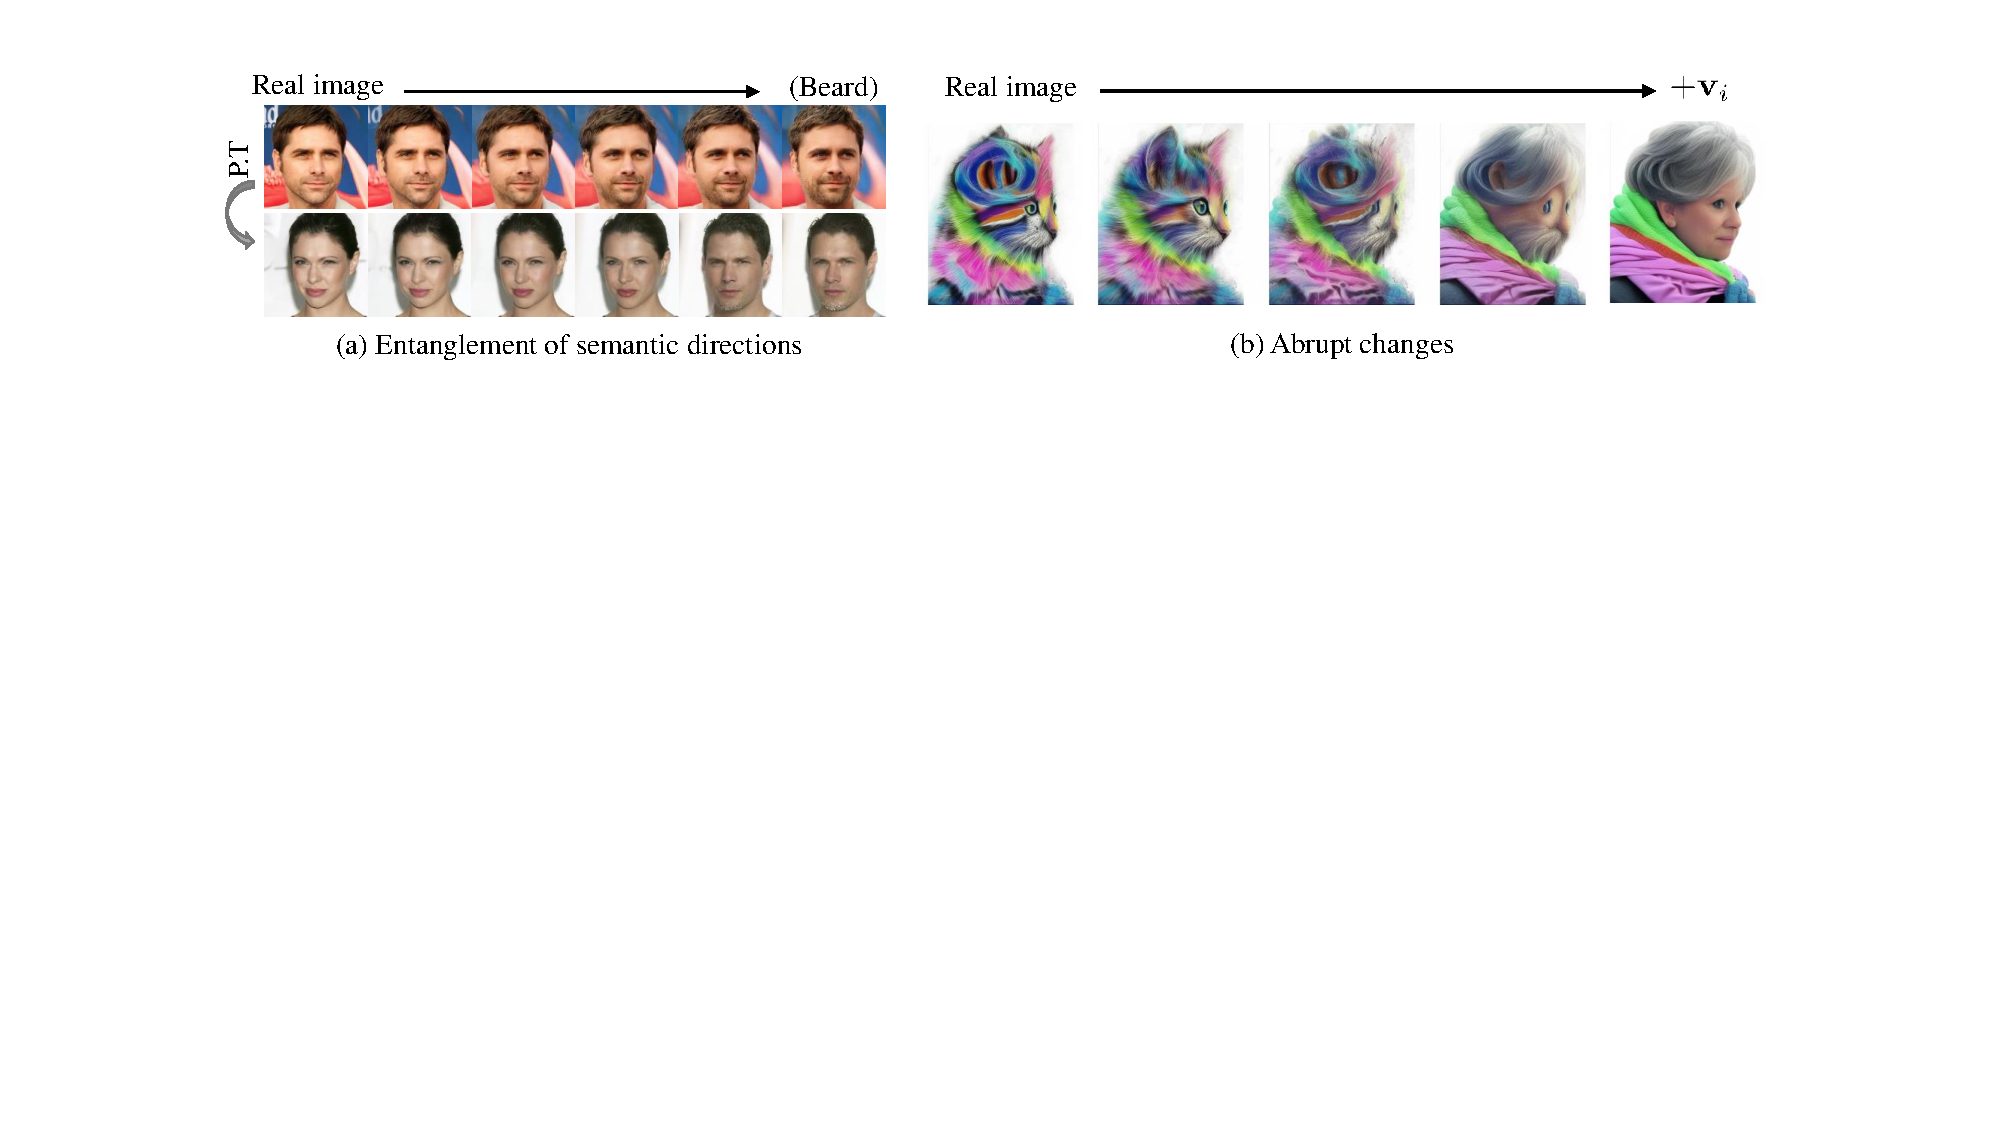
\includegraphics[width=1.0\linewidth]{figure/limitation.pdf}
    \vspace{-1.5em}
    \caption{
    \textbf{Limitations.} (a) Entanglement between attributes due to \jo{dataset biases}
    %the dataset prior. 
    (b) Abrupt changes in Stable Diffusion.}
    \vspace{-1em}
    \label{fig:limitation}
\end{figure}

While our method has shown effectiveness in Stable Diffusion, more research is needed to fully validate its potential.
We have observed that some of the discovered latent vector occasionally leads to abrupt changes during the editing process in Stable Diffusion, as depicted in Figure \ref{fig:limitation} (b). 
% In contrast to GANs, where changes tend to occur continuously, we often encounter instances where the transformations appear more like the result of crushing objects, manifesting as discontinuous changes. 
This observation highlights the complex geometry of $\mathcal{X}$ in achieving seamless editing. Exploring this topic in future research is an interesting area to delve into.

\modify{
Our approach is broadly applicable when the feature space in the DM adheres to a Euclidean metric, as demonstrated by \(\mathcal{H}\). This characteristic has been observed in the context of U-Net within \citet{kwon2022diffusion}. It would be intriguing to investigate if other architectural designs, especially those similar to transformer structures as introduced in \cite{peebles2023scalable, tevet2022human}, also exhibit a Euclidean metric.
}



% Although we have shown that our method is also valid to Stable Diffusion, we still need more observation. It discovers less number of latent latent directions and few directions occasionally convey abrupt changes during the editing procedure in Stable Diffusion as shown in \fref{fig:limitation} (b). We suppose that its learned latent space may have a more complex manifold than the image space \cite{arvanitidis2017latent}. Alternatively, the conditional DMs with classifier-free guidance or the cross-attention mechanism may add complexity on the manifold. Our future work includes analyzing the latent directions in the conditions such as text prompts or segmentation labels.

Despite these limitations, our method provides a significant advance in the field of image editing for DMs, and provides a deep understanding of DM through several experiments.

% \vspace{-0.5em}
\section{Conclusion}
\vspace{-0.5em}
We have analyzed the latent space of DMs from a geometrical perspective. 
We used the pullback metric to identify the latent and tangent bases in $\mathcal{X}$ and $\mathcal{H}$. 
The latent basis found by the pullback metric allows editing images by traversal along the basis.
% We can edit images by traversal along the latent directions.
We have observed properties of the bases in two aspects.
% We investigated the discovered structure from two aspects.
% First, we examined how the latent structure changes over time, and 
First, we discovered that 1) the latent bases evolve from low- to high-frequency components; 2) the discrepancy of tangent spaces from different samples increases along the generative process; and 3) DMs trained on simpler datasets exhibit more consistent tangent spaces over timesteps.
Second, we investigated how the latent structure changes based on the text conditions in Stable Diffusion, and discovered that similar prompts make tangent space analogous but its effect becomes weaker over timesteps.
We believe that a better understanding of the geometry of DMs will open up new possibilities for adopting DMs in useful applications.

\vspace{-0.5em}
\section{Acknowledgement}
\vspace{-0.5em}
\jo{This work was supported in part by the Creative-Pioneering Researchers Program through Seoul National University, the National Research Foundation of Korea (NRF) grant (Grant No. 2022R1A2C1006871) (J. J.)}, KIAS Individual Grant [AP087501] via the Center for AI and Natural Sciences at Korea Institute for Advanced Study, and the National Research Foundation of Korea (NRF) grant (RS-2023-00223062).


